\noindent
\begin{tabular}{cc}
\begin{minipage}{0.60\textwidth}
\begin{exerciseS}[Getto libero]
Si consideri un getto stazionario, assialsimmetrico, d'acqua in 
condizioni standard, diretto verso l'alto, in atmosfera uniforme, 
secondo la verticale $z$, e uscente con velocit\`{a} uniforme e 
costante $V = 20\ m/s$ da un ugello circolare di diametro 
$d = 5\  cm$. Si assuma che:
\begin{itemize}
\item la curvatura delle linee di flusso sia trascurabile;
\item sia trascurabile ogni perdita di energia.
\end{itemize}
Si determinino:
\begin{itemize}
\item[a)] il diametro $D$ del getto alla quota $Z = 15\ m$
          (misurata dal piano d'uscita dall'ugello);
\item[b)] la massima quota ideale $H$ cui pu\`{o} giungere il getto.
\end{itemize}
($D = 6.97\ cm$, $H = 20.39\  m$)
\end{exerciseS}
\end{minipage}
&
\begin{minipage}{0.35\textwidth}
   \begin{center}
   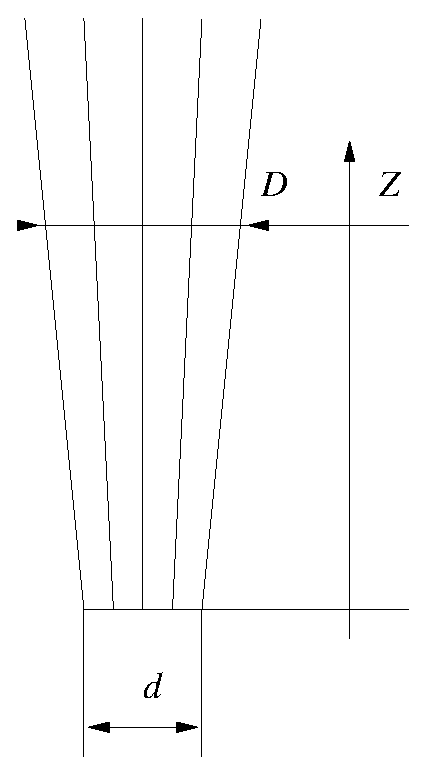
\includegraphics[width=0.60\textwidth]{./fig/getto_vert.eps}
   \end{center}
\end{minipage}
\end{tabular}

\sol

\partone
 Teorema di Bernoulli nell'ipotesi di stazionarietà, fluido incomprimibile, non viscoso, irrotazionale.
Equazione della vorticità nel caso non viscoso.

\parttwo

\begin{itemize}
\item Il primo quesito del problema viene risolto mettendo a sistema l'equazione di
 Bernoulli (ipotesi...) e l'equazione della continuità.
\begin{equation}
\begin{cases}
  \frac{1}{2} \rho V^2  = \frac{1}{2}\rho u^2(z) + \rho g z\\
  V d^2 = u(z) D^2
\end{cases} \qquad \Rightarrow \qquad D = \frac{d}
{\displaystyle\left[1 - \frac{2 g z}{V^2}\right]^{\frac{1}{4}}}
\end{equation}
 Inserendo i valori numerici $D = 6.97 \text{cm}$.

\item Il secondo quesito si ottiene ricavando dal teorema di Bernoulli la quota alla quale 
la velocità è nulla.

\begin{equation}
  \frac{1}{2} \rho V^2 = \rho g H \qquad \Rightarrow \qquad 
  H = \frac{1}{2} \frac{V^2}{g}
\end{equation}
 Inserendo i valori numerici $H = 20.39 \text{m}$.

\end{itemize}


